\scanpage{104}
\diagram{\begin{tikzcd}k&V\arrow[l]\arrow[r]&K\end{tikzcd}}
\margin{\figure{\begin{tikzpicture}\node[draw,ellipse,rotate=15]{\uuline{parfait} ?};\end{tikzpicture}}}
\diagram{\begin{tikzcd}[column sep=large]
\mathcal K\operatorname{Gr}_K\arrow[d,"T"'] &
\text{complexes finis de \deleted{\unsure{quasi}} $K$-groupes \deleted{\unsure{alg}}}\\
\unsure{K|\mathcal K}\operatorname{QuGr}_k & \text{complexes finis de $k$-quasi-groupes}
\end{tikzcd}}
\margin{\deleted{$\unsure{T^0}$}}
\margin{[Coh de $K$. \uline{ne se calcule pas} galoisiennement]}
\margin{[Coh. de $k$ se calcule galoisiennement, \deleted{\unsure{et}}
ne change pas en remplaçant $k$ par une clôture \unsure{parfaite}]}
\[
T(G)=T^0_{\unsure{a}}e(G)
\]
\[
\Gamma^*_{\unsure{K}}G\simeq\Gamma^0_K e(G)
\simeq\Gamma^0_k T^0e(G)\simeq\Gamma^*_kT(G)
\]
\deleted{\unsure{Question}}\figure{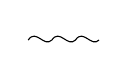
\begin{tikzpicture}\draw(0,0)..controls(.1,.15)and(.2,-.1)..(.3,0)..controls(.4,.15)and(.5,-.1)..(.6,0)..controls(.7,.15)and(.8,-.1)..(.9,0);\end{tikzpicture}}
\noindent (i) $T^0$ transforme injectifs en $\Gamma^0_k$-acycliques ??

\noindent (ii) $T^0$ de dim coh. $\leq2$
[et même $\leq1$ si on \deleted{\unsure{excepte}}\inserted{exclut}
les composantes de type $\mathbb Z$]

\noindent (iii) $T^*$ commute à ``\uline{l'extension du corps résiduel $k$}''.

i.e est ``de nature géométrique'' ;
\diagram{\begin{tikzcd}[column sep=large,row sep=small]
\underline{\underline H}^*(K,G^\bullet) &
H^p(k,\underline{\underline T}^{\unsure{q}}(G^\bullet))\arrow[l,Rightarrow]\\
\underline{\underline H}^*(k,T(G))\arrow[u,equal]&
\end{tikzcd}}
\[
\left[\begin{aligned}
\underline{\underline{\operatorname{Ext}}}^{\unsure{\bullet|*}}_{K\text{-gr}}(F,G)
&\Longleftarrow H^p(k,\underset{\sim}{\underline{\operatorname{Ext}}}^q_{K/k}(F,G))\\
&\Longleftarrow H^p(K,\underset{\sim}{\underline{\operatorname{Ext}}}^q_K(F,G))
\end{aligned}\right.
\]
\mspage{103}

